\chapter{Tapaus: Sovelia PLM:n raportointityökalu} \label{Tapaus: Sovelia PLM:n raportointityökalu}

\section{Sovelia PLM} \label{Sovelia PLM}

Kehitettävän raportointityökalun toimintaympäristönä toimii kaupallinen PLM-järjestelmä, Sovelia PLM. Sovelia PLM:n kehitys on alkanut yli 30 vuotta sitten ja sen kehitys jatkuu aktiivisesti edelleen. Kuten muutkin PLM-järjestelmät, Sovelia PLM pyrkii ratkaisemaan valmistusalan yritysten haasteita liittyen tuotteen datan hallintaan sen koko elinkaaren ajan. \cite{soveliaAboutSovelia} Sovelia PLM:n erityispiirteenä on sisältämät valmiiksi konfiguroidut \textit{"templatet"} eli valmiit mallit objekteille ja prosesseille, jotka ovat muokattavissa asiakkaan tarpeiden mukaan. Lisäksi malleihin kuuluu muita valmiiksi konfiguroituja työkaluja että alalla hyväksi todettuja prosesseja. \cite{soveliaSoveliaGetting}

Sovelia PLM koostuu objekteista ja objektilinkeistä. Objekteja voidaan määritellä niiden attribuuttien avulla. Objektit voivat olla osia, piirustuksia, dokumenttilinkkejä tai linkkejä muihin toimintoihin. \cite{soveliaSoveliaGetting} Objektilinkkien avulla voidaan muodostaa osaluetteloita, jotka ovat tärkeitä raportoinnin kohteita. Näiden lisäksi toinen merkittävä konsepti Soveliassa on käyttäjä ja käyttäjäryhmät. Yksinkertaisuudessaan järjestelmällä voi olla luonnollisesti useita käyttäjiä ja käyttäjät voivat kutsua eri käyttäjäryhmiin. Käyttäjäryhmiä voi olla useita, mutta tärkein niistä on ymmärtää \textit{"admin"}-ryhmä (engl. \textit{administrator}), johon kuuluu pääkäyttäjät eli järjestelmänvalvojat. Järjestelmänvalvojalla on luonnollisesti oikeuden muuttaa järjestelmän asetuksia. Pääkäyttäjän konsepti on tärkeä ymmärtää, sillä osa kehitettävän raportointityökalun ominaisuuksista on saatavilla vain pääkäyttäjälle. Käyttäjäryhmien lisäksi jokaisella käyttäjällä on lisenssi, joka määrittelee osaltaan käyttäjän oikeuksia rajoittamalla esimerkiksi objektien ja objektilinkkien muokkausoikeuksia. \cite{soveliaUserManagement}

\subsubsection{Raportointi Sovelia PLM-järjestelmässä} \label{Raportointi Sovelia}

Sovelia PLM ja muut PLM-järjestelmät poikkeavat valmiiden raportointityökaluratkaisujen tyypillisistä toimintaympäristöistä, sillä kuten luvussa \ref{PLM-järjestelmä toimintaympäristönä} huomattiin, PLM-data on usein kompleksista ja monimuotoista. Siemensin PLM-järjestelmän verkkosivuilla \cite{german_challenge_2016} julkaistussa artikkelissa \textit{"The Challenge of Getting High Quality Reports out of PLM"} esitellään haasteita, joita liittyy korkealaatuisten raporttien tuottamiseen PLM-järjestelmistä. Artikkeli nostaa esille osaluetteloiden (BOM) merkityksen PLM-järjestelmän raportoinnissa: on tärkeää että raporttien saama ja tuottama data on luotettavaa ja laadukasta, jotta päätöksenteko raporttien pohjalta olisi mahdollista. Osaluetteloihin voi tulla jopa satoja muutoksia päivittäin, joten raporttien tapauksessa on tärkeää, että niiden käyttäjät tietävät työskentelevänsä oikean datan kanssa. Täten raporttien ajantasaisuus ja selkeät aikaleimat ovat hyvin tärkeitä PLM-järjestelmän ja myös Sovelian tuottamille raporteille. Sovelia PLM:n raportointimoottorin etuna on hakurajapinnan käyttö, joka palauttaa aina hakupyynnön mukaisesti ajankohtaista dataa, mikä vähentää mahdollisten virheellisten tietojen määrää. \cite{german_challenge_2016}

PLM-datan kompleksisuus tekee raportointityökalun kehittämisestä haasteellista, sillä myös Sovelia PLM vaatii erityisesti tarkoitusta varten kehitetyn raportointityökaluratkaisun. Tarkoitusta varten kehitetty ratkaisu on ohjelmistokehittäjälle työläs rakentaa alusta asti itse, mutta sen etuna on sen täysi muovautuvuus tarvetta varten. On kuitenkin todettava, että myös valmiin raportointimoottorin ja -työkalun implementoiminen Sovelia PLM:n toimintaympäristöön olisi todennäköistä työlästä juuri PLM-datan kompleksisuuden vuoksi.

\subsubsection{Sovelia PLM:n vanha raportointityökalu}

Sovelia PLM -järjestelmässä on tuotannossa ja asiakkailla käytössä vanha raportointiyökalu, joka tarjoaa raportteja PDF, Excel ja ZIP-tiedostoformaateissa. Näistä poikkeavimpia ovat ZIP-raportit eli ZIP-arkistot, \nomenclature[ZIP]{ZIP}{tiedon pakkaukseen käytetty tiedostomuoto, joka voi sisältää useita tiedostoja ja kansioita pakattuna} jotka sisältävät useita PDF- tai Excel-raportteja pakattuna yhteen tiedostoon. Täten ZIP-raporttiin voidaan sisällyttää esimerkiksi raportti tuoterakenteen jokaiselle yksittäiselle objektille, jolloin ZIP-paketin kansiorakenne vastaa itsessään tuotteen rakennetta. Raporttidokumenttein data kerätään \textit{"rakenneagentin"} avulla, joka on nimensä mukaisesti osaa kulkea objekti-linkki -suhteita pitkin ja täten kerätä tarvittavan lähdedatan raportin koostamista varten. Itse raporttidokumentteihin kirjoittaminen tapahtuu Java-ohjelmointikielen Apache FOP-ohjelmakirjaston \cite{noauthor_apachetm_nodate} avulla XSL-\nomenclature[XSL]{XSL}{XML-kieliperhe, joka mahdollistaa XML-pohjaisten tiedostojen ulkoasun ja rakennemuutoksen määrittelyn} (engl. \textit{Extensible Stylesheet Language}, kieliperhe, joka mahdollistaa XML-pohjaisten tiedostojen ulkoasun ja rakennemuutoksen määrittelyn) ja XML-tietorakenteisiin tallennetun datan antaman ohjeistuksen avulla.

Vaikka tämä ratkaisu on toimiva ja edelleen kelvollinen tekniikka dokumenttien muotoiluun, ja siten raporttien generointiin ohjelmallisesti ennalta määritellyn datan mukaisesti, se kohtaa ongelmia datamäärien kasvaessa. Näihin ongelmiin kuuluu esimerkiksi liiallinen muistinkäyttö palvelimella, prosessin hitaus varsinkin suurempien tuoterakenteiden tapauksissa ja raporttien konfiguroinnin haasteellisuus sen ollessa täysin mahdotonta PLM-järjestelmän loppukäyttäjille. Lisäksi toiminnon ylläpito alati muuttuvassa toimintaympäristössä muuttuu todennäköisesti haasteellisemmaksi tulevaisuudessa, kun uusi teknologia syrjäyttää vanhaa yhä useammilla osa-alueilla, samalla kun vanhalle pohjalle rakennettu raportointimoottori ei pysy samalla tavalla muutoksen tahdissa.

\subsubsection{Uuden raportointityökalun haasteet} \label{Uuden haasteet}

Koska vanhan raportointityökalun modernisointi ja päivittäminen nykypäivään vaatisi perustavanlaatuisia muutoksia koko järjestelmään, päädyttiin valitsemaan kehityskohteeksi kokonaan uuden raportointityökalun kehittämisen. Uuden työkalun tarkoituksena on integroitua paremmin nykyiseen Web-pohjaiseen käyttöliittymään ja tarjota käyttäjäystävällisemmän kokemuksen raporttien luomiseen. Raporttien luominen tuoterakenteista tapahtuisi käyttäjän näkökulmasta paremmin integroituna Web-käyttöliittymään tarjoten mahdollisuuden seurata meneillään olevien raporttien edistymistä sekä perua raporttien koostamisprosesseja käyttöliittymästä käsin. Lisäksi pääkäyttäjällä tulisi olla mahdollisuus muokata ja luoda uusia raporttityyppejä muokkaamalla esimerkiksi raporteissa esitettäviä sarakkeita ja tuoterakenteiden suodattamiseen liittyviä sääntöjä. Myös raporttien ulkonäön tulee olla muokattavissa pääkäyttäjän toimesta, mikä tarkoittaa niiden visuaalisen ilmeen muokkausta lisäämällä asiakasyrityksen logoja, muokkaamalla väriteemaa ja asettelua asiakkaan tarpeiden mukaisesti.

Uuden raportointityökalun tulee ensimmäisessä vaiheessa sisältää samat toiminnallisuudet kuin vanha raportointityökalu, mutta tarkoituksena on tuottaa raportteja huomattavasti nopeammin aiheuttamalla samanaikaisesti vähemmän kuormaa palvelimelle. Raporttien sisällön ja yleisen rakenteen tulee vastata vanhempia raportteja identtisesti, mutta raporttien visuaalinen ilme tulee päivittää nykypäivän standardien mukaiseksi. Lisäksi vaaditaan syvällisiä teknologiatutkimusta ja -analyysiä olemassa olevien raportointityökalujen ja -moottorien ratkaisuista, Sovelia PLM:n ohjelmakannassa jo olemassa olevista komponenteista ja muista mahdollisesti hyödyllisistä teknologioista.

\section{Nykyiset erilliset raportointityökalut} \label{Nykyiset erilliset}

Ennen käytettävien teknologioiden ja tekniikoiden valintaa on hyvä perehtyä jo olemassa oleviin raportointityökaluihin ja -moottoreihin, jotta voidaan muodostaa kokonaiskuva yleisesti käytössä olevista ratkaisuista. Hyvän kokonaiskuvan avulla voidaan tehdä valistuneita päätöksiä siitä, miten raportointityökalua kannattaa lähteä kehittämään sekä ymmärtää käytössä olevien tekniikoiden hyötyjä ja rajoituksia PLM-järjestelmän kontekstissa. Analysoimme kuutta suosittua itsenäistä (engl. \textit{standalone}) raportointityökalua, joista neljä ovat kaupallisia ja kaksi ovat avoimen lähdekoodin ohjelmistoja. Juuri nämä kuusi raportointityökalua valittiin tarkasteltavaksi, sillä ne ovat kaikki paikallisesti asennettavia ohjelmistoja (engl. \textit{On-premise software}) kuten myös Sovelia PLM. Täten tässä tutkimuksessa ei keskitytä esimerkiksi ulkoisten pilvipalveluiden raportointityökalu verkko-ohjelmointirajapintoihin (engl. \textit{Web API}). Yksi esimerkki tällaisesta verkkopohjaisesta API:sta on \textit{Bold Reports} \cite{noauthor_bi_2022}, joka tarjoaa monipuolisen verkkorajapinnan kautta toimivan raportointityökalun. Toinen kriteeri tarkasteluun valinnalle oli käytettävä teknologia, sillä Sovelia PLM:n nykyinen arkkitehtuuri nojaa vahvasti Java- ja JavaScript-ohjelmointikieliin, joten täysin uuden ohjelmointikielen lisäämistä järjestelmäarkkitehtuurin pinoon ylläpidettäväksi ei pidetty mielekkäänä vaihtoehtona. Lisäksi esimerkkejä sekä Java- että JavaScript-pohjaisia raportointityökaluista löytyi runsaasti, joten uuden teknologian valitseminen ei vaikuttanut välttämättömyydeltä. Kolmas tärkeä kriteeri oli ulostulodataformaattien monipuolisuus: koska Sovelia PLM -järjestelmään kehitettävän raportointityökalun tulee tuottaa raportteja eri tiedostoformaateissa, tulee myös tarkasteltavien työkalujenkin.

Puhtaasti kaupallisia ohjelmistoja ovat JavaScript-pohjainen \textit{ActiveReportsJS}, SAP:in, maailman suurimman yritysohjelmistoja tarjoavan yrityksen \cite{noauthor_sap_nodate-3}, kaksi raportointityökalua \textit{SAP Business Objects} ja \textit{SAP Crystal Reports} ja Oraclen, talouslehti Forbesin mukaan vuoden 2023 80. suurimman julkisen yrityksen \cite{tucker_global_nodate}, raportointityökalu \textit{Orancle BI Publisher}. Vahva esimerkki taas avoimen lähdekoodin vaihtoehdosta on \textit{JasperReports}, joka kutsuu itseään suosituimmaksi avoimen lähdekoodin Java-raportointikirjastoksi. \cite{noauthor_jasperreports_nodate}. \textit{JasperReports} sisältää myös visuaalisen suunnittelutyökalun, \textit{iReport Designerin}, joten \textit{JasperReports} on kokonainen raportointityökaluohjelmisto. \textit{JasperReports} sisältää myös vaihtoehtoisen maksullisen lisenssin yrityskäyttöön tarjoten yritysasiakkaille parempaa tukea ja ratkaisua suuremman skaalan raportointiin. \cite{noauthor_jasper_nodate} Toinen avoimen lähdekoodin raportointityökalu on myös Java-pohjainen \textit{BIRT} (lyhenne engl. \textit{"Business Intelligence Reporting Tool"}), joka tarjoaa monipuolisia raportointimahdollisuuksia täysin avoimen lähdekoodin ja Eurooppalaisen \textit{Eclipse Foundationin} ylläpitämä ohjelmisto. \cite{eclipsebirtBIRT} \textit{BIRT} on keskittynyt raportoinnin lisäksi myös Business Intelligencen hyödyntämiseen asiakas- ja web-applikaatioissa, joten se sisältää monia erilaisia visualisointimahdollisuuksia ja raportointimoottorin lisäksi myös graafisen raporttikonfigurointityökalun.

\subsubsection{Nykyisten raportointityökalujen yleiskuva} \label{Nykyisten yleiskuva}

Raportointityökalua kehittääkseen osaksi PLM-järjestelmää varten tulee lisenssien lisäksi ottaa huomioon myös muita ominaisuuksia. Liitteenä olevassa taulukossa \ref{tab:Yleista} luokitellaan raportointiyökalujen yleisiä ominaisuuksia. Taulukoiden data on kerätty taulukossa mainituista lähteistä, kuten ohjelmiston verkkosivuilta, ohjelmakirjaston dokumentaatiosta tai myyntiesitteistä. Jo mainitut lisenssit ovat eritelty kaupallisiin ja avoimen lähdekoodin ohjelmistoihin. Avoimen lähdekoodin ohjelmistot tarjoavat asiantuntijoille lähdekoodin perehtymisen avulla syvän katsauksen raportointityökalun sisäiseen toiminnallisuuteen, mutta tässä tutkimuksessa keskitymme enemmän pintapuolisempiin ominaisuuksiin ja teknologiavalintoihin tarkemman lähdekoodianalyysin sijasta. Yksi tällaisista ominaisuuksista on lähdedatan formaatti ja mahdolliset datalähteet. Kaikki tutkitut raportointityökalut tukivat jotakin rakenteellisen datan tallentamiseen suunniteltua tiedostoformaattia eli tässä tapauksessa XML:ää tai JSON:ia. Ainoastaan \textit(ActiveReportsJS) ei tukenut XML:ää, mutta se tukee kuitenkin JavaScript-pohjaisena luonnollisesti JSON:ia. Rakenteellisen datan tukeminen tärkeää varsinkin PLM:n datan tapauksessa, jossa objektien ja siten tuotteiden väliset suhteet ovat avainasemassa. Näiden tiedostoformaattien lisäksi noin puolet tarkasteltavista raportointityökaluista tuki myös SQL-kyselyitä tietolähteenä \nomenclature[SQL]{SQL}{engl. \textit{Structured Query Language}, standardoitu kyselykieli, jolla relaatiotietokantaan voi tehdä erilaisia hakuja, muutoksia ja lisäyksiä} (engl. \textit{Structured Query Language}). Näiden lisäksi myös tavallisten tekstitiedostojen käyttö tietolähteenä on tyypillistä XML- ja JSON-tiedostojen lisäksi, kuten myös Excel-taulukkolaskentaohjelman tuottamat XLSX-tiedostot. Mielenkiintoista on, että myös Excelin tuottamat XLSX-tiedostot koostuvat itseasiasiassa vain ZIP-pakatuista XML-tiedostoista. \cite{miner_under_2022}

Raportointityökalujen ohjelmointikieliä tarkastellessa suosituimmaksi ilmeni Java, sillä kaikki paitsi \textit(ActiveReportsJS) olivat Java-pohjaisia. Yksi syy tähän voi olla Javan suuri ja vakaa suosio 1990-lopussa ja 2000-luvun alussa ohjelmointikielten suosiota mittaavan \textit{TIOBE indexin} mukaan\cite{noauthor_tiobe_nodate}, jolloin suurinta osaa näistä raportointityökaluista alettu kehittää. Esimerkiksi \textit{JasperReportsia} on alettu kehittää vuonna 2001 \cite{noauthor_origin_2006}, \textit{BIRTiä} vuonna 2004 \cite{noauthor_eclipse_2004} ja \textit{BusinessObjectsia} jo vuonna 1995 ennen kuin se kuului SAP-tuoteperheeseen \cite{alma9922048891805971}. Kuten {TIOBE indexistä} voidaan havaita, on Java edelleen suhteellisen suosittu kieli käyttää vuonna 2023, mutta sen suosio on kuitenkin jo hieman laskussa. Raporttipohjien konfigurointi tapahtuu raportointityökaluissa pääsääntöisesti jonkin käyttöliittymän avulla. Käyttöliittymän lisäksi \textit{ActiveReportsJS} tarjoaa mahdollisuuden konfiguroida raporttipohjia JSON-datan avulla, \textit{BIRT} ja  \textit{JasperReports} XML-datan avulla ja \textit{Oracle BI Publisher} RTF (engl. \textit{Rich Text Format}, eroaa tavallisesta tekstistä tallentamalla tiedostoon myös fontit, fonttikoot ja yleisen muotoilun, mm. kursivoinnin) ja XSL-pohjaisesti. Tästä voidaan havaita, että visuaalinen käyttöliittymä raporttipohjien luomiselle on suosituin tapa toimia, mutta tiedostopohjainen raporttipohjien muokkaus on käypä vaihtoehto.

\subsubsection{Nykyisten raportointityökalujen ulostuloformaatit}

Raportointityökalun tärkein tehtävä on tuottaa raportteja, jolloin raporttien tulee olla myös helposti avattavissa ja esitettävissä eri laitteilla. Liitteenä olevassa taulukossa \ref{tab:Formaatit} tarkastellaan samojen kuuden raportointityökalun tarjoamia ulostuloformaatteja, eli sitä millaisissa tiedostomuodoissa työkalut tarjoavat raportteja. Ulostuloformaattien valinta on erityisen tärkeää raportointityökalulle, sillä sen käyttäjät suosivat heille jo entuudestaan tuttuja tiedostomuotoja, sekä ohjelmistoteknisestä näkökulmasta, sillä raporttien tuottaminen erilaisissa tiedostomuodoissa vaatii usein tiedostomuotokohtaisia työkaluja.

Tiedostomuodot voidaan jaotella avoimiin ja suljettuihin tiedostomuotoihin. Avoimessa tiedostomuodossa olevan tiedoston avaaminen on mahdollista ilman kaupallista ohjelmaa, jolloin se on kenen tahansa avattavissa ja sillä on avoimesti saatavilla oleva spesifikaatio. \cite{fileformats} Suljettu tiedostomuoto on luonnollisesti avoimen tiedostomuodon vastakohta, jolloin spesifikaatio ei ole avoimesti saatavilla. Suljettu tiedostomuoto voi olla hyödyllinen joissain tapauksissa, esimerkiksi silloin jos tiedostoon tulee tallentaa tai sen avulla tulee esittää dataa siten että muut esimerkiksi avoimet tiedostomuodot eivät siihen pysty. Avoimien tiedostomuotojen suosiminen on kuitenkin kannattavaa, sillä se vähentää riippuvuutta kolmannen osapuolen ohjelmistoista tai tiedostomuotojen lisenssinhaltijoista. Pahimmassa tapauksessa tietoja voidaan lukea vain tietyillä ohjelmistopaketeilla, jotka voivat olla kohtuuttoman kalliita tai jotka voivat vanhentua. \cite{fileformats}

Ulostuloformaateista erityisen suosittu on Adoben kehittämä PDF (engl. \textit{Portable Document Format}), jota käytetään erityisesti sähköiseen julkaisemiseen. PDF on ollut ISO-standardi vuodesta 2007 alkaen ja ISO (engl. \textit{International Organization for Standardization}, kansainvälinen standardisoimisjärjestö) kuvailee sitä maailman suosituimmaksi dokumenttitiedostoformaatiksi \cite{naden_standard_2021}. Vaikka PDF on alun perin Adoben kehittämä kaupallinen ja suljettu tiedostomuoto, on sen spesifikaatio ISO-standardoinnin jälkeen avoimesti saatavilla. Suosionsa, standardoinnin ja avoimen spesifikaation vuoksi PDF onkin luonnollinen valinta raportointityökalun ulostuloformaatille ja siksi myös kaikki kuusi tarkastelevaa raportointityökalua tarjoavat raportteja PDF-muodossa.

Raporttidokumenteille selkeästi suosittuja alustoja ovat erityisesti yritysmaailmassa suositun Microsoft Officen tuottamat tiedostomuodot, erityisesti taulukkolaskentaohjelma Excelin \textit{.xlsx} ja \textit{.xls} ja tekstinkäsittelyohjelma Wordin tuottamat \textit{.docx} ja \textit{.doc} tiedostot. Microsoft Officen tiedostomuotojen laaja tuki raportointityökalujen saralle ei ole varsinaisesti yllättävää ottaen huomioon, että tilastopalvelu \textit{Statistan} mukaan Microsoftilla on noin 45 prosentin markkinaosuus toimisto-ohjelmistojen alalla Googlella sen ollessa noin 50. \cite{office} On kuitenkin otettava huomioon, että myös Google tarjoaa omissa toimisto-ohjelmistoissaan mahdollisuuden avata ja muokata myös Microsoft Officen tuottamissa tiedostomuodoissa olevia tiedostoja. Sekä Excelin että Wordin tuottamat tiedostomuodot \textit{.xlsx} ja \textit{.docx} ovat suljettuja tiedostomuotoja, mutta ne ovat kuitenkin Googlen tarjoamien työkalujen lisäksi avattavissa esimerkiksi avoimen lähdekoodin ohjelmistolla LibreOfficella \cite{libreoffice}. Täten vaikka Word ja Excel-tiedostot ovat suljetussa tiedostomuodossa, on ne mahdollista avata ilman kaupallisia ohjelmistoja. Microsoft Officen tiedostomuodoista erityisesti taulukkomuotoisten raporttien tapauksessa Excelin \textit{.xlsx}-tiedostot ovat hyödyllisiä, sillä ne tarjoavat raportointityökalun käyttäjälle mahdollisuuden tutkia raportin sisältöä vielä pintaa syvemmältä suorittamalla itse laskentaa ja kokoamalla kuvaajia ohjelman avulla. Raportteja Excel- ja Word-tiedostoformaateissa tarjosivat kaikki tarkasteltavat raportointityökalut paitsi ActiveReportsJS, eli nämä formaatit ovat PDF-raporttien ohella erityisen suosittuja.

Kolmas suosittu tiedostomuoto on HTML (engl. \textit{Hypertext Markup Language}, suom. \textit{hypertekstin merkintäkieli}) \nomenclature[HTML]{HTML}{engl. \textit{HyperText Markup Language}, suom. \textit{hypertekstin merkintäkieli}, merkintäkieli, jolla internetsivut ovat kirjoitettu}, joka on erityisesti verkkosivujen kirjoittamisessa käytetty merkintäkieli. HTML ei ole ohjelmointikieli vaan merkintäkieli, joka määrittelee miten sisältö tulisi muotoilla. Myös HTML on avoin ja ISO-standardoitu tiedostomuoto.\cite{iso_html} HTML:ää käytetään usein yhteydessä CSS:n kanssa (engl. \textit{Cascacing Style Sheets}, suom. \textit{porrastetut tyyliarkit}) \nomenclature[CSS]{CSS}{engl. \textit{Cascacing Style Sheets}, suom. \textit{porrastetut tyyliarkit}, tyylisivu, jolla voidaan määritellä tyyliohjeita miten esimerkiksi HTML dokumentti voidaan esittää}. CSS on eräänlainen tyylisivu, jolla voidaan määritellä tyyliohjeita siitä, miten esimerkiksi HTML dokumentti voidaan esittää. Kuten HTML myöskään CSS ei ole ohjelmointikieli, mutta se tarjoaa valtavasti mahdollisuuksia muotoilla HTML-dokumentteja. HTML:n ja CSS:n ohella verkkosivut hyödyntävät tyypillisesti myös JavaScriptia. HTML-raportit tarkoitettu esitettäväksi verkkoselaimessa, mikä tekee niistä hyvin alustariippumattomia. Mikäli HTML-raportit sisältävät CSS-tyyliarkin ja JavaScriptia, näitä hyödyntämällä HTML raportteihin voidaan lisätä animaatioita ja muita toiminnallisuuksia, ne voivat olla huomattavasti interaktiivisempia käyttäjälle verrattuna staattisempiin PDF-, Excel ja Word-raporttidokumentteihin. HTML-pohjaisia raportteja tarjosivat poikkeuksetta kaikki tarkasteltavat kuusi raportointityökalua.

Viimeisenä ulostuloformaattina vain \textit{SAP BusinessObjects} ja \textit{SAP Crystal Reports} mahdollistavat raporttien tuottamisen näiden raportointityökalujen omassa suljetussa tiedostomuodossa nimeltä \textit{RPT}, joka lyhennelmä englannin kielen sanasta \textit{report}. Koska \textit{RPT} tiedostoformaatti on suljettu ja se ei ole yleisesti laajalti käytössä oleva tiedostoformaatti, \textit{SAP BusinessObjectsin} ja \textit{SAP Crystal Reportsin} ulkopuolella, sen avaaminen on käytännössä mahdollista vain tätä varta vasten kehitetyllä ohjelmalla toisin kuin esimerkiksi Word- ja Excel-tiedostojen tapauksessa.

\section{Uuden raportointityökalun kehitys} \label{Uuden kehitys}

Ensimmäinen haaste raportointityökalun kehittämiselle on käytettävien tekniikoiden ja teknologioiden valinta. Koska tarkoituksena on kehittää täysin uusi toiminnallisuus alusta alkaen, on tärkeää ymmärtää nykyiset Sovelia PLM:ssä käytössä olevat komponentit palvelinarkkitehtuurien näkökulmasta. Itse raportointimoottorin täytyy toimia jollakin palvelimella ja koostaa valmiit raportit palvelinpäässä ennen niiden lataamista käyttäjien saataville. Tällä menettelyllä voidaan vähentää asiakaspään kuormaa siirtämällä raskaampi laskenta palvelimen vastuulle. Palvelinpäässä kuormaa voidaan tasata asettamalla tehtävät jonoon odottamaan suoritusvuoroaan.

\subsubsection{Uuden raportointimoottorin palvelinympäristö}

Tarkastelemalla olemassa olevia raportointityökaluja, Java osoittautui suosituimmaksi ohjelmointikieleksi raportointityökalun ohjelmointirajapinnalle. Luvussa \ref{Nykyisten yleiskuva} kuitenkin todettiin, että Java on suosioltaan laskussa \textit{TIOBE Indexin} mukaan vuonna 2023. Sovelia PLM hyödyntää ohjelmistopinossaan (engl. \textit{software stack}) Java-palvelinta, mutta se on elinkaareltaan enemmänkin ylläpitovaiheessa, eikä sen alaisuuteen ole suunnitelmissa kehittää kokonaan uusia toiminnallisuuksia. Uuden raportointityökalun tarkoituksena on olla mahdollisimman tulevaisuudenkestävä (engl. \textit{future-proof}), joten on olennaista tarkastella myös vaihtoehtoisia palvelinympäristöjä raportointityökalulle.

Raportointimoottorin palvelinympäristöksi valiutui lopulta Sovelia PLM:ssä jo käytössä oleva Node.js, joka on avoimen lähdekoodin alustariippumaton ajoympäristö JavaScript-koodin suorittamiseen erityisesti palvelinympäristössä. Node.js oli vuoden 2023 Stack Overflown teettämän kyselyn mukaan yleisin käytetty Web-teknologia ammattikehittäjien keskuudessa React.js:n ohella noin 42 prosentin käyttöasteella. \cite{stackoverflowStackOverflow} Kyselyn mukaan Node.js on kuitenkin vuoden 2023 johtava teknologia palvelinpuolella, sillä React.js on tarkoitettu enemmänkin käyttöliittymien kehittämiseen asiakaspäässä. Node.js tarjoaa ohjelmistokehittäjälle oletuksena paketinhallintajärjestelmän nimeltään NPM (engl. \textit{Node Package Manager, NPM}, tyyliteltynä npm), joka koostuu komentorivityökalusta ja JavaScript -ohjelmapaketteja ylläpitävästä tietokannasta. NPM:n avulla erillisten ohjelmakirjastojen sisällyttäminen ja käyttöönotto on yksinkertaista ja nopeaa.\cite{npmjsAbout} Node.js:n suosion vuoksi käytettävissä on laaja kattaus erilaisia hyödyllisiä ohjelmakirjastoja. NPM helpottaa erityisesti tarvittavien ohjelmakirjastojen käyttöönottoa ja asennusta, joita raportointimoottori tarvitsee erityisesti raporttidokumenttien kokoamiseen ohjelmallisesti. Sovelia PLM:n Node.js-palvelimen tarkoituksen oli erilaisia palveluita ja rajapintoja Sovelia PLM:n Web-käyttöliittymälle. Näihin palveluihin kuuluu esimerkiksi 3D-näkymien ja -tiedostojen tarjoaminen Web-käyttöliittymälle, joten myös raportointimoottorin sisällyttäminen samalle palvelimelle oli luonteva ratkaisu, sillä myös raporttien konfigurointityökalu sekä toiminnot raporttien suorittamiseen tullaan kehittämään Sovelia PLM:n web-käyttöliittymään.

\subsubsection{Uuden raportointityökalun ominaisuuksia}

Datalähteenä Sovelia PLM:n uusi raportointimoottori käyttää Node.js pohjaisena JSONia, joka oli käytössä myös muissa tarkastelluissa raportointityökaluissa. Luvussa \ref{Nykyisten yleiskuva} todettiin JSONin olevan hyvä valinta hierarkkisen PLM-datan tallentamiseen. Luvun \ref{Raportointimoottorin rakenne ja prosessi} alaluvussa koskien logiikkatasoa huomattiin JSONin olevan nopeampi verrattuna vanhempaan XML-standardiin \cite{nurseitov_comparison_nodate}. Uusi raportointityökalu hyödyntää lähdedatan hankkimisessa Sovelia PLM-järjestelmän olemassa olevaa hakumoottoria, joka palauttaa itsessään JSON-muotoista dataa, joten muuntamisvaihetta erilliseen dataformaattiin ei tarvita.

\begin{figure}[tbh]
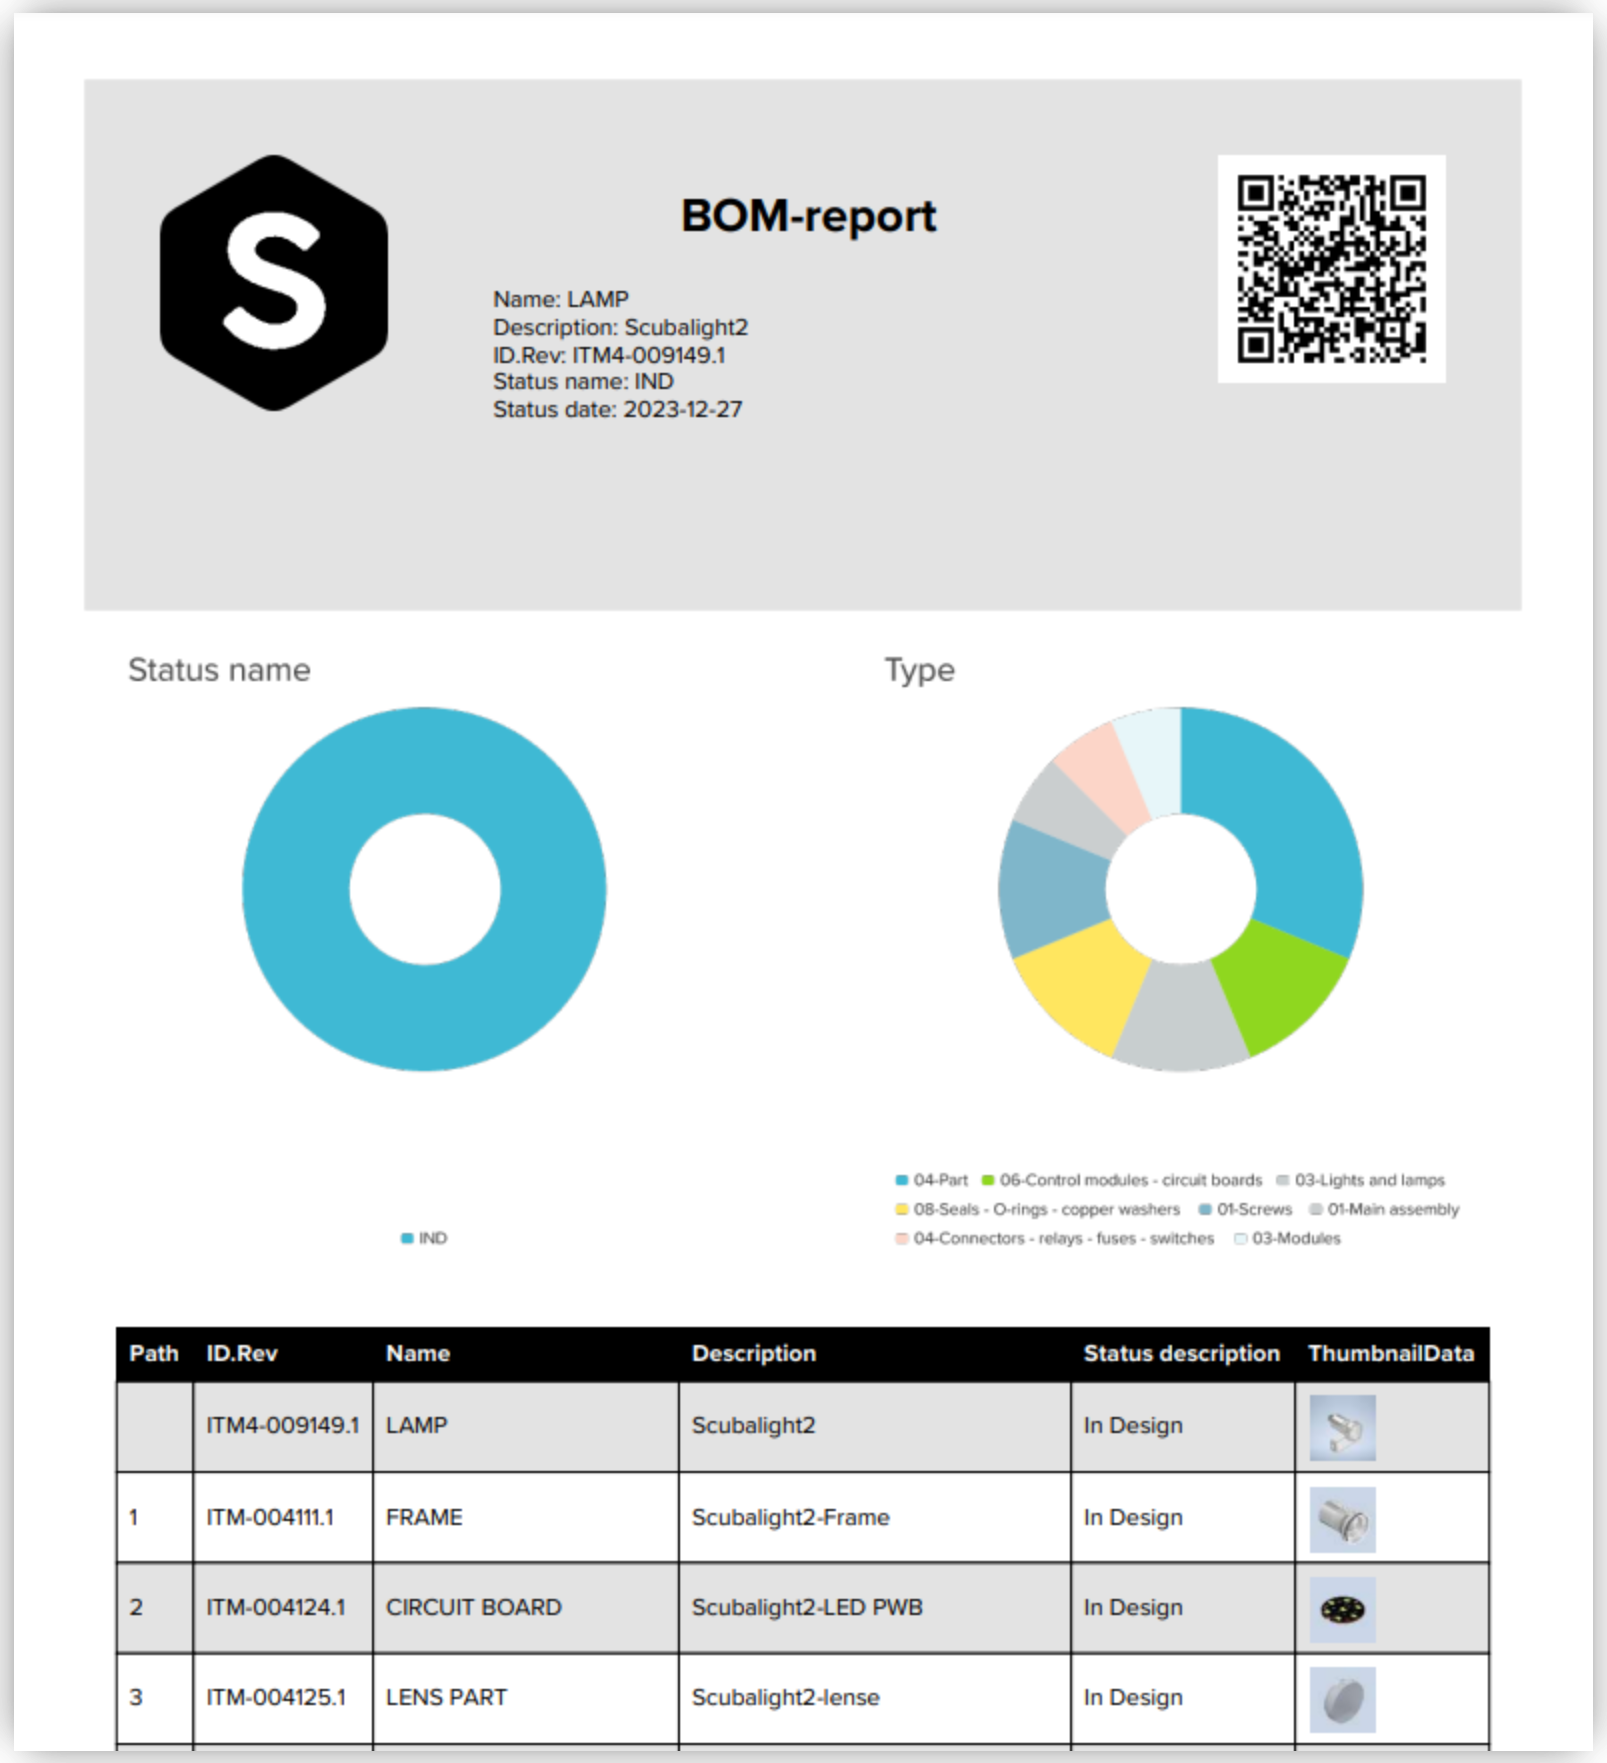
\includegraphics[width=1\textwidth]{img/report.png}
\caption{Kuvakaappaus Sovelia PLM:n raportointimoottorin tuottamasta BOM-raportista PDF-muodossa\label{fig:report}}
\end{figure}

Sovelia PLM:n uusi raportointityökalu tuottaa raportteja PDF-, Excel ja ZIP-muodoissa eli se tukee tarkasteltujen raportointityökalujen suosituimpia formaatteja. PDF-raportit tarjoavat taulukoidun tuotedatan lisäksi myös piirakkakuvaajia tuoterakenteen eri tietokenttien arvojen jakaumasta, Excel-raportit mahdollistavat rakenteellisen esittämisen tasoittain ja tarjoavat laskentamahdollisuuksia. ZIP-raportit ovat taas kokoavat tuoterakenteesta useita PDF- tai Excel-raportteja ja lisäävät arkistoon myös tuoteobjektien liitetiedostoja, kuten piirustuksia. Uusi raportointimoottori tukee myös HTML-raportteja, mutta ne eivät kuulu ensimmäisen version vaatimusmäärittelyyn, eivätkä siten ole osa ensimmäistä julkaistavaa versiota.

\begin{figure}[tbh]
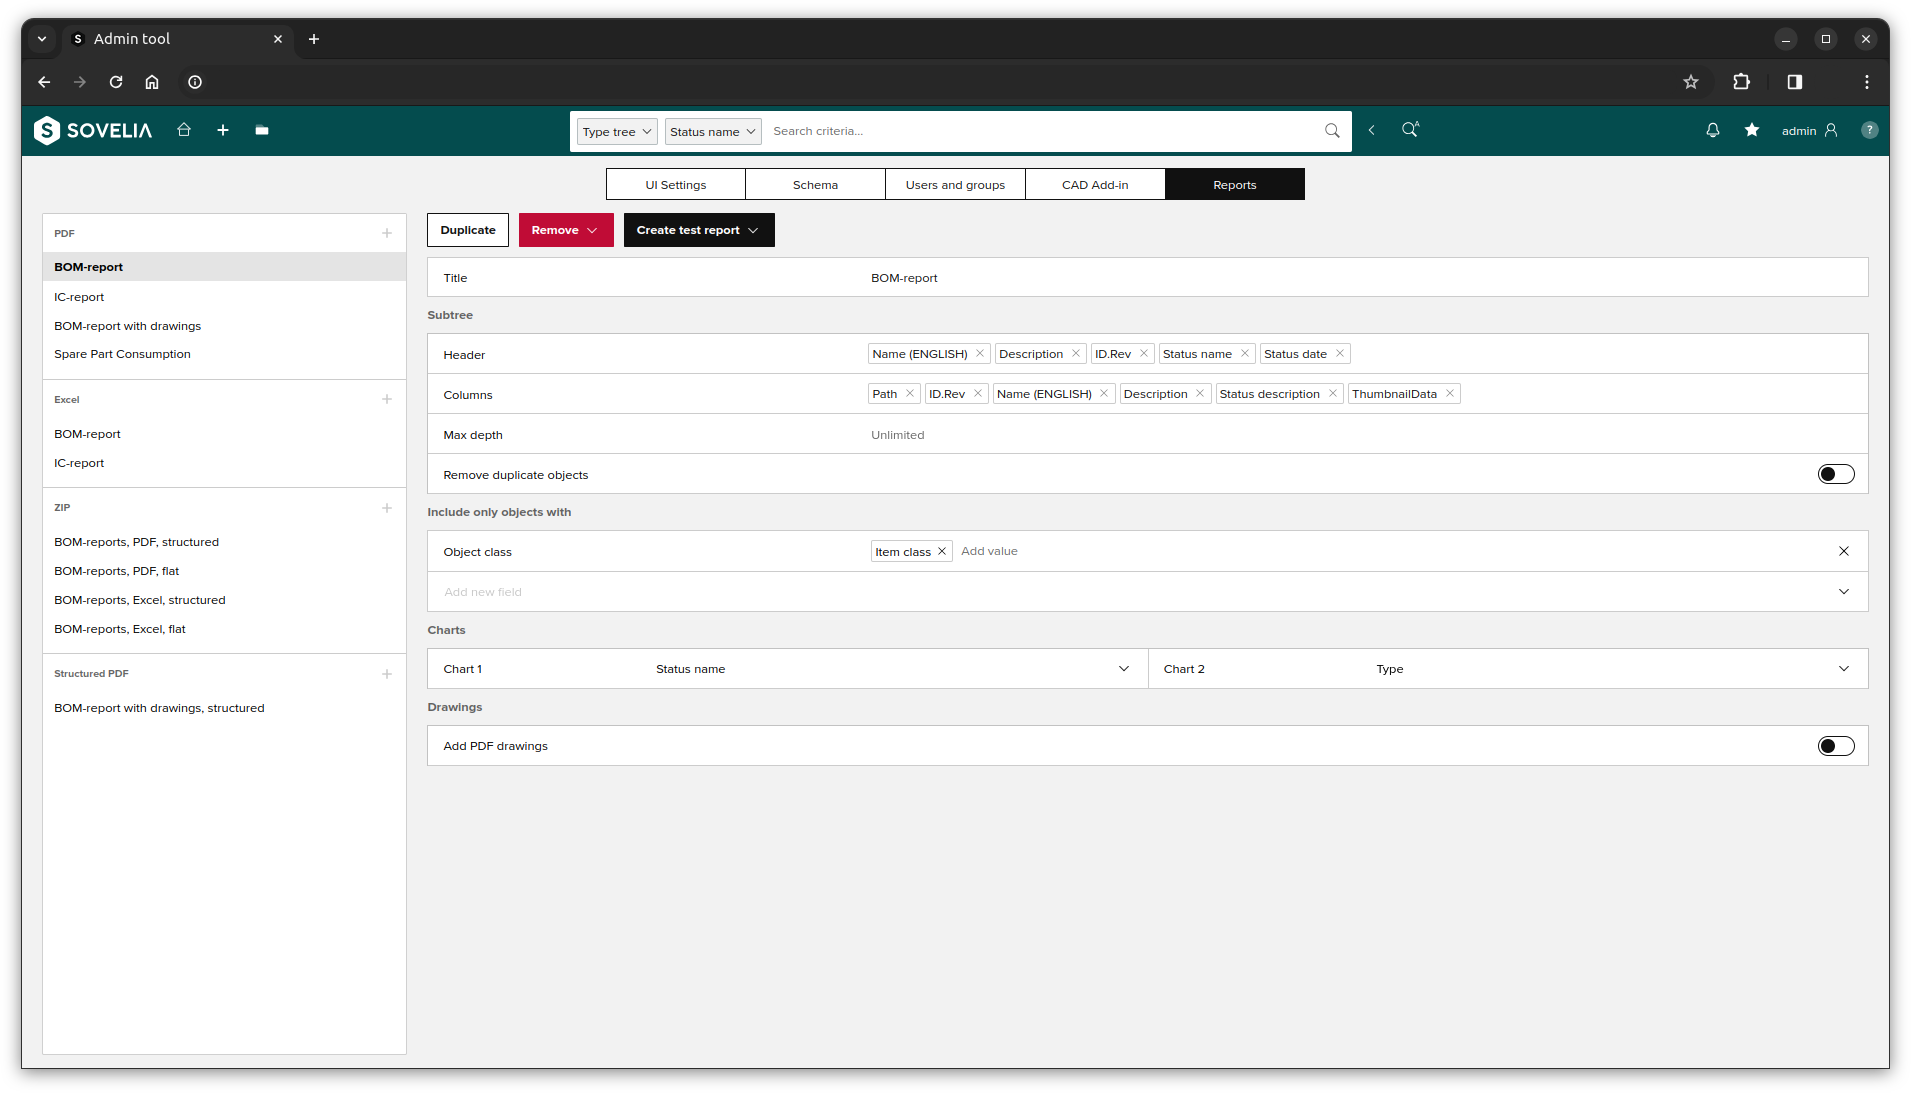
\includegraphics[width=1\textwidth]{img/RAT.png}
\caption{Kuvakaappaus Sovelia PLM:n raportointityökalun Web-käyttöliittymän kehitysversiosta\label{fig:RAT}}
\end{figure}

Raporttipohjien konfigurointi tapahtuu uudella raportointityökalulla tapahtuu Sovelia PLM:n web-käyttöliittymässä pääkäyttäjän toimesta. Käyttöliittymässä voidaan luoda, muokata ja poistaa raportteja, sekä säätää interaktiivisten valikoiden avulla esimerkiksi tietokentät, joista muodostetaan raportin kuvaajat ja taulukot. Raportointimoottori osaa myös laskea lisäkenttiä, kuten esimerkiksi osien kokonaissummia tuoterakenteessa. Tuoterakenteista voidaan myös suodattaa pois määritellyn ominaisuuden mukaisesti tuoteobjekteja, tai raportissa esitettävä tuoterakenne voidaan asettaa koostumaan vain tietyn ominaisuuden omaavista tuoteobjekteista. ZIP-raporttipaketteihin voidaan valita halutut tuoteobjektien liitetiedostojen tiedostomuodot. Myös PDF-raportteihin on mahdollista liittää tuotteiden ja osien piirustuksia PDF-muodossa. ZIP-paketin "aliraportiksi" voidaan valita mikä tahansa järjestelmään konfiguroitu Excel- tai PDF-raportti. Aliraportilla tarkoitetaan tässä raporttia, joka ajetaan käyttöliittymässä annettujen kriteerien mukaisesti tuoterakenteen eri alirakenteille tai osille.

% Kuva ZIP-raportin rakenteesta?

\subsubsection{Uuden raportointityökalun tulevaisuus}

Uusi raportointimoottori Node.js -palvelimella on osoittautunut testausvaiheessa tehokkaaksi ja nopeaksi keinoksi muodostaa raportteja. Suoritusajat ovat huomattavasti vanhaa raportointityökalua nopeampia ja muistinkäyttö palvelimella on vähäisempää. Konfigurointia on pyritty tekemään loppukäyttäjille helpommaksi tarjoamalla graafinen Web-käyttöliittymä raporttien konfigurointiin ja raportteja voidaan luoda suoraan Sovelia PLM:n valikoista. Tulevaisuuden ominaisuuksina on tarkoitus kehittää graafinen suunnittelutyökalu PDF-raporteille, lähettää monitorointidataa raportointimoottorin suorituskyvystä sekä tarjota loppukäyttäjille enemmän mahdollisuuksia vaikuttaa raporttien ulkoasuun.

